Bathymetry is a measurement of submarine topography and can be used to understand shifts of the ocean floor and its depth. Knowledge of bathymetry is important for marine navigation, both civilian and military, as well as for monitoring and predicting the effects of storms on coastal environments. While direct measurement of bathymetry is possible, the process tends to be cost and time prohibitive. For example, amphibious vehicles are capable of spatially limited surveys of bathymetry in difficult surf-zone conditions but require significant resources to operate. As a result of these factors, surveys tend to be sparse in time. 

The research we conducted for this report focuses on a method to estimate bathymetry, using surface measurements collected via remote sensing platforms, i.e. airborne, satellite, or onshore platforms. While bathymetry data is currently sparse due to observational limitations, the physics of waves are reasonably well understood. In particular, a dispersion relationship can be used to relate water depth to surface properties such as wave length and wave period. This relationship makes it possible to estimate bathymetry given the observations of these parameters. Light Detection And Ranging (LiDAR) has been used to determine wave heights and Argus land-mounted video has been analyzed photogrammetrically to determine wave frequency and wave number. Moreover, these resources  provide valuable inputs for estimating coastal bathymetry in a more efficient manner than is currently available.

Wave and bathymetric data has been collected in Duck, NC by the U.S. Army Corps of Engineers Coastal and Hydraulics Laboratory, including in situ measurements of bathymetry and measurements of the water surface. These measurements provide a method for testing algorithms to invert for bathymetry because the true bathymetry is available for comparison to the numerical estimates.

We invert for depth, \textit{h}, using wave number with a 1D model derived using the energy flux method to create a correlation between wave length and depth from the water surface as shown in Figure~\ref{flowchart}.
\begin{figure}[H]
		\centering
		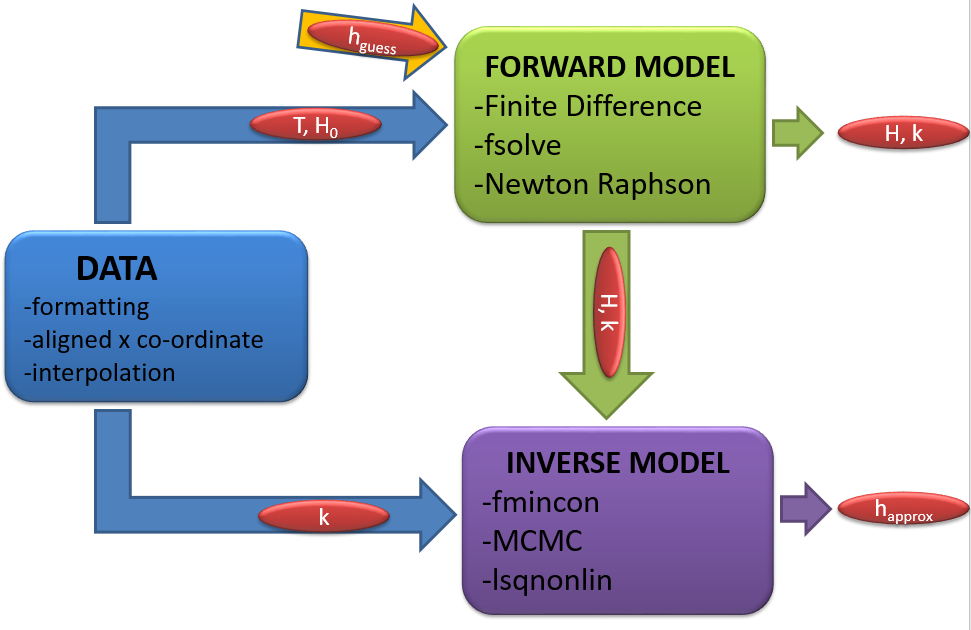
\includegraphics[width=.90\linewidth]{img/Flow_Chart.png}
		\caption{Flow chart of the workflow for this research}
		\label{AWAC}
\end{figure}
In section 2 we discuss about how data is observed and use to measure different wave parameters. In section 3 we discuss about the forward problem and numerical results of forward problem. Inversion method is discussed in section 4 with discussion related the methods applied. In the last section 5 we discuss about the experimental results. These results were generated using both simulated and real data using some existing tools.